\subsection{Интеграл Фруллани.}
\begin{lemma}
    Пусть $f \in C([0, +\infty))$ и для любого $A > 0 \hookrightarrow$
    \[
        \int_A^{+\infty} \dfrac{f(x)}{x}dx
    \]
    сходится в несобственном смысле.
    Тогда $\forall a, b > 0$ справедлива формула Фруллани:
    \[
        I = \int_0^{+\infty} \frac{f(ax) - f(bx)}{x}dx = f(0)\ln \frac{b}{a}.
    \]
\end{lemma}
\begin{proof}
    Поскольку
    \[
        I = \lim\limits_{\epsilon \ra +0, E \ra +\infty} \int_{\epsilon}^{E} \dfrac{f(ax) - f(bx)}{x}dx.
    \]
    Введём обозначение:
    \[
        I(\epsilon, E) = \int_{\epsilon}^{E} \dfrac{f(ax) - f(bx)}{x}dx.
    \]
    Поскольку
    \[
        I(\epsilon, E) = \int_{\epsilon}^E \dfrac{f(ax)}{x}dx - \int_{\epsilon}^{E} \dfrac{f(bx)}{x}dx = \int_{a\epsilon}^{aE} \dfrac{f(t)}{t}dt - \int_{b\epsilon}^{bE} \dfrac{f(t)}{t}dt = \int_{a\epsilon}^{b\epsilon} \dfrac{f(t)}{t}dt + \int_{bE}^{aE} \dfrac{f(t)}{t}dt = J(\epsilon) + K(E).
    \]
    Ключевой момент заключается в том, что $K(E) \ra 0, E \ra +\infty$ -- это следует из критерия Коши сходимости в применении к несобственному интегралу, данному в условии.
    А $J(\epsilon)$ оценивается как
    \[
        J(\epsilon) = \int_{a\epsilon}^{b\epsilon} \dfrac{f(t) - f(0)}{t}dt + \int_{a \epsilon}^{b\epsilon} \dfrac{f(0)}{t}dt = f(0) \ln \frac{b}{a} + \int_{a\epsilon}^{b\epsilon} \dfrac{f(t) - f(0)}{t}dt \ra f(0) \ln \frac{b}{a}.
    \]
    Второе слагаемое стремится к 0 из непрерывности $f$:
    \[
        \biggr|\int_{a \epsilon}^{b\epsilon} \dfrac{f(0)}{t}dt \biggr| \leq \sup\limits_{t \in [a\epsilon, b \epsilon]}|f(t) - f(0)| \ln \frac{b}{a} \ra 0, \epsilon \ra +0.
    \]
\end{proof}
\begin{example}
    Рассмотрим интеграл $I = \int_0^1 \frac{x^\alpha - x^\beta}{\ln x}dx$.
    Сделаем замену $x = e^{-t}$ и получим
    \[
        I = -\int_0^{+\infty} \dfrac{e^{-\alpha t} - e^{-\beta t}}{t} e^{-t}dt = \ln \dfrac{a + 1}{b + 1}.
    \]
    с использованием формулы Фруллани к функции $f(t) = e^{-t}$.
\end{example}
\subsection{Интеграл Дирихле}

\[
    \int\limits_0^{+\infty} \frac{\sin x}{x} \, dx \text{ ~---~ интеграл Дирихле}
\]

\begin{note}
Понимаем как несобственный интеграл Лебега
\end{note}

\begin{theorem}
\[
    \int\limits_0^{+\infty} \frac{\sin x}{x} \, dx = \frac{\pi}{2}
\]

\end{theorem}

\begin{proof}

\noindent Сделаем регуляризацию, то есть добавим множитель, чтобы из несобственного интеграла получить собственный. 

\noindent Рассмотрим функцию:

\[
F(x, y) := \frac{\sin x}{x} \cdot e^{-x y}, \ x, y \in [0, +\infty)
\]

\[
F(x, 0) = \frac{\sin x}{x},
\]

\noindent Заметим, что $F$ ~---~ непрерывная как функция двух переменных. Доопределим в нуле:
\[
F(0, 0) = 1,  
\]

\noindent Тогда функция непрерывна на $[0, +\infty) \times [0, +\infty)$. 

Рассмотрим интеграл (зависящий от параметра): 
\[
D(y) := \int\limits_0^{+\infty}F(x, y) \,d x
\]


\noindent Формально продифференцируем по параметру
\[
    D'(y) = \int\limits_0^{+\infty} \frac{d}{dy} \left( e^{-x y} \right) \cdot \frac{\sin x}{x} \, dx = - \int\limits_0^{+\infty} e^{-x y} \cdot \sin x \, dx
\]

\noindent Из формулы Эйлера $e^{ix} = i \sin x + \cos x$:

\[
D'(y) = -\mathrm{Im} \int\limits_0^{+\infty} e^{-xy} \cdot e^{ix} \, dx
= -\mathrm{Im} \int\limits_0^{+\infty} e^{-x(i - y)}\, dx
= -\mathrm{Im} \left( \left. \frac{e^{-x(i - y)}}{i - y} \right|_0^{+\infty} \right) = -\mathrm{Im}\left( 0 - \frac{1}{i-y}\right) =
\]

\[
= \mathrm{Im} \left( \frac{1}{i - y} \right) = \mathrm{Im} \left( \frac{-i - y}{1 + y^2} \right)
= \frac{-1}{y^2 + 1}
\] 

\noindent Итого:
\[
D'(y) = \frac{-1}{y^2 + 1}, y > 0
\]

\[
\forall\, y_1, y_2 > 0 \text{ при } y_2 > y_1 \quad
D(y_2) - D(y_1) = \int\limits_{y_1}^{y_2} D'(y) \, dy
= - \int\limits_{y_1}^{y_2} \frac{1}{y^2 + 1} \, dy = \arctan{y_1} - \arctan{y_2}
\]

\noindent При $y_2 \to +\infty$:

\[
D(y_2) = \int\limits_0^{+\infty} \frac{\sin x}{x} \cdot e^{-x y_2} \, dx
\]

Возьмем под модуль:

\[
\left| D(y_2) \right| 
= \left| \int\limits_0^{+\infty} \frac{\sin x}{x} \cdot e^{-x y_2} \, dx \right|
\leq \int\limits_0^{+\infty} e^{-x y_2} \, dx
= \frac{1}{y_2} \longrightarrow +0, \  y_2 \to +\infty
\]



\noindent Перейдем к пределу при $y_2 \rightarrow + \infty,  y_1 \rightarrow +0$: 

\[
- \lim_{y_1 \to +0} D(y_1) = -\frac{\pi}{2} \Rightarrow \lim_{y_1 \to +0} D(y_1) = \frac{\pi}{2}
\]

\begin{note}
Если доказать, что $D(y)$ непрерывен в нуле справа, то есть что $\lim_{y \to +0} D(y) = D(0)$, то получим искомое
\end{note}

\noindent Покажем, что \( D(y) \) — непрерывна и существует \( D'(y) \), \( \forall y > 0 \).

\noindent Зафиксируем произвольные \( y_1, y_2 \), такие что \( 0 < y_1 < y < y_2 \)

\begin{center}
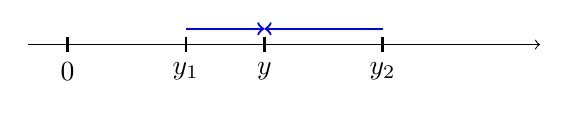
\begin{tikzpicture}
    \draw[->] (-0.5,0) -- (6,0); % ось
    \foreach \x/\label in {0/0, 1.5/\(y_1\), 2.5/\(y\), 4/\(y_2\)} {
        \draw[thick] (\x,0.1) -- (\x,-0.1) node[below] {\label};
    }
    \draw[->, thick, blue] (1.5,0.2) -- (2.5,0.2); % стрелка y1 -> y
    \draw[->, thick, blue] (4,0.2) -- (2.5,0.2);   % стрелка y2 <- y
\end{tikzpicture}
\end{center}


\begin{note}
Чтобы можно было дифференцировать по $y$, достаточно проверить, что интеграл $D(y)$ сходится $\forall y > 0$ и что $- \int\limits_0^{+\infty} \sin x \cdot e^{-x y} \, dx$ сходится равномероно по $y$.
\end{note}

\noindent Очевидно, что $ \sin x \cdot e^{-x y}$ непрерывна на $[y_1, y_2] \times [0, +\infty)$.

\noindent $\frac{\sin{x}}{x}\cdot e^{-x y}$, доопределенная в нуле тоже непрерывна на $[y_1, y_2] \times [0, +\infty)$.


\[
\left| \frac{\sin x}{x} \cdot e^{-x y} \right| \leq e^{-x y}
\]

\[
 \Rightarrow \frac{\sin x}{x} \cdot e^{-x y} \in L_1([0, +\infty)) \quad \text{(принадлежит $L_1$ как функция от } x\text{) \,} \forall y > 0
\]

\[
\Rightarrow D(x) \, \text{сходится} \, \forall y > 0
\]


\noindent Назовем $J(y) = - \int\limits_1^{+\infty} \frac{\sin x}{x}  e^{-x y} \, dx$. (от 1 потому что так будет проще применить признак Дирихле)

\noindent Покажем, что $J(y)$ сходится равномерно по $y$ на $[y_1, y_2]$


\noindent Воспользуемся признаком Дирихле:
\begin{enumerate}


    \item 

\[
\sup_{y > 0} \sup_{A} \left| \int_{1}^{A} \sin x \, dx \right| \leq 2 
\]

    \item 
\[
\frac{e^{-x \cdot y}}{x} \downarrow 0, \quad x \to +\infty \quad \forall y > 0
\]

    \item 
\[
0 \leq \frac{e^{-x y}}{x} \leq \frac{e^{-x \cdot y_1}}{x} \rightarrow 0, x \rightarrow + \infty\, \forall y \in [0, y_2], \forall x > 1 \Rightarrow
\]


\[
\sup_{y \in [0, y_2]} e^{-x y} \to 0, \ x \to +\infty.
\]


\noindent $\Rightarrow$ В силу признака Дирихле $ \int_{1}^{+\infty} \frac{\sin x}{x} \, e^{-x y} \, dx $ сходится равномерно по $y$

\noindent В силу признака Вейерштрасса 
$
\int_{0}^{+\infty} \sin x \, e^{-x y} \, dx \quad \text{сходится равномерно по } y \in [y_1, y_2]
$

\[
|\sin x \, e^{-x y}| \leq e^{-x \cdot y_1}, \quad \int_{0}^{+\infty} e^{-x \cdot y_1} \, dx \quad - \text{сход.}
\]



\end{enumerate}


\noindent Это доказывает, что можно дифференцировать интеграл по параметру при любом $y > 0$


\noindent $\int_{1}^{+\infty} \frac{\sin x}{x} \, e^{-x y} \, dx $ сходится равномерно по $y$ 

\noindent $\Rightarrow  \int_{0}^{+\infty} \frac{\sin x}{x} e^{-x y} \, dx \quad \text{сходится равномерно по } y \in [0, y_2] \quad \forall y_2 > 0. $

\begin{note}
Мы доказали от 1 до $+\infty$. Но интеграл от 0 до $+\infty$ отличается минимально:
\end{note}
\[
\text{На } [0, 1] \times [0, y_2] \text{ функция } F(x, y) = \frac{\sin x}{x} e^{-x y} \text{ непрерывна по совокупности переменных.}
\]

\noindent Тогда, следующие условия эквивалентны: 

\begin{enumerate}
    \item \(\int\limits_0^{+\infty} \frac{\sin x}{x} \, e^{-x y} \, dx \) сходится равномерно по \( y \) на множестве \( [0, y_2] \).
    
    \item \(\int\limits_1^{+\infty} \frac{\sin x}{x} \, e^{-x y} \, dx \) сходится равномерно по \( y \) на множестве \( [0, y_2] \).
\end{enumerate}

\noindent Равномерную сходимость мы требуем, чтобы обосновать непрерывность в нуле. 

\noindent Запишем условия для перехода к пределу по параметру. 

\begin{enumerate}
    \item $\int\limits_0^{+\infty} \frac{\sin x}{x} \, e^{-x y} \, dx$ сход. равномерно по $y$ на $[0, y_2 ] \ \forall y_2 > 0.$

    \item $\frac{\sin x}{x} = \lim\limits_{y \to +0} e^{-x y} \frac{\sin x}{x}.$


    \item В силу непрерывности: 
    $$
    F: e^{-x y} \frac{\sin x}{x} \mathrel{\substack{\rightrightarrows \\ [0, t]}} \dfrac{\sin x}{x}  \ \forall t > 0 \Rightarrow \int\limits_{0}^{t} e^{-xy} \dfrac{\sin x}{x} dx \rightarrow \int\limits_{0}^{t} \dfrac{\sin x}{x} dx \ \forall t > 0.
    $$
    
\end{enumerate}

\noindent Все эти условия выполнены. Тогда существует предел: 

\[
\int\limits_0^{t} e^{-x y} \frac{\sin x}{x} \, dx 
\longrightarrow.
\int\limits_0^{t} \frac{\sin x}{x} \, dx \quad \forall\, t > 0.
\]


\[
\Rightarrow \exists \lim_{y \to +0} \int\limits_0^{+\infty} \frac{\sin x}{x} \, e^{-x y} \, dx 
= \int\limits_0^{+\infty} \frac{\sin x}{x} \, dx.
\]
А это и означает непрерывность функции $D$ в нуле справа.

\noindent Тогда  все переходы в настоящем доказательстве обоснованы и интеграл Дирихле полностью посчитан. 

\end{proof}


\section{Преобразование Фурье}
\begin{definition}
Пусть $f \in L_1^{loc}(\R)$.
Преобразованием Фурье функции $f$ будем называть функцию $\mathcal{F}[f]$, которая $\forall x \in \R$ определяется как
\[
    \mathcal{F}[f](x) := \dfrac{1}{\sqrt {2\pi}}\vpint_{\R} f(y)e^{-ixy}dy.
\]
\end{definition}

\begin{note}
\textbf{v.p.} (от фран. \textit{Valeur Principale})~---~интеграл в смысле главного значения по Коши.
\[
\vpint_{\mathbb{R}} f(y) e^{-ixy}dy := \lim_{A \to +\infty} \int\limits_{-A}^{A} f(y)e^{-ixy}dy.
\]
\end{note}

\begin{definition}
    Обратное преобразование Фурье определим как
    \[
        \mathcal{F}^{-1}[f](x) := \dfrac{1}{\sqrt {2\pi}}\vpint_{\R} f(y)e^{ixy}dy.
    \]
\end{definition}

\begin{note}
    Для интегрируемых на всей числовой прямой функций интеграл в смысле главного значения совпадает c обычным интегралом Лебега.
\end{note}

\begin{note}
    Ключевым отличием интеграла в смысле главного значения от несобственного интеграла Лебега являются симметричные пределы интегрирования.\\
    Нетрудно заметить, что интеграл в смысле главного значения от любой нечётной функции $g \in L_1^{loc}(\R)$ будет равен $0$:
    \[
        \forall A \in \R \hookrightarrow \int_{-A}^{A} g dx = 0 \Ra \vpint_{\R} gdx = 0.
    \]
\end{note}
\subsection{Интеграл Фурье}
\begin{question}
Нас будет интересовать вопрос: для каких функций обратное преобразование Фурье действительно является <<обратным>> преобразованием? То есть
\[
    \mathcal{F}^{-1}[\mathcal{F}[f]] = \mathcal{F}[\mathcal{F}^{-1}[f]] = f.
\]
На первый взгляд кажется, что всегда.
Однако не все так просто.
\end{question}
\begin{definition}
    введём следующее обозначение $\forall A > 0$:
    \[
        I_A[f](x) = \dfrac{1}{\sqrt {2\pi}} \int_{-A}^{A} \mathcal{F}[f](y)e^{ixy}dy.
    \]
\end{definition}

\begin{lemma}[Ключевая]\label{lem:key}
Пусть $f \in L_1(\mathbb{R})$ и $x \in \mathbb{R}$. Тогда $\forall A > 0$ справедливо равенство:
\[
I_A \left[ f \right](x) = \int\limits_{-\infty}^{+\infty} f(x - t) \frac{\sin(At)}{\pi t} \, dt.
\]
\end{lemma}

\begin{proof}

Заметим, что $F(y, u) = f(u)e^{i(x-u)y}$ интегрируема на множестве $(-A, A) \times \mathbb{R}$ при любом фиксированном $x \in \mathbb{R}$:
\[
    \iint\limits_{(-A, A) \times \R} |f(u)e^{i(x - u)y}|dxdy \leq \int_{-A}^{A}dy \int_{\R}|f(u)|du = 2A \int_{\R} |f(u)|du < +\infty.
\]

%\begin{figure}[h!]
%    \centering
%    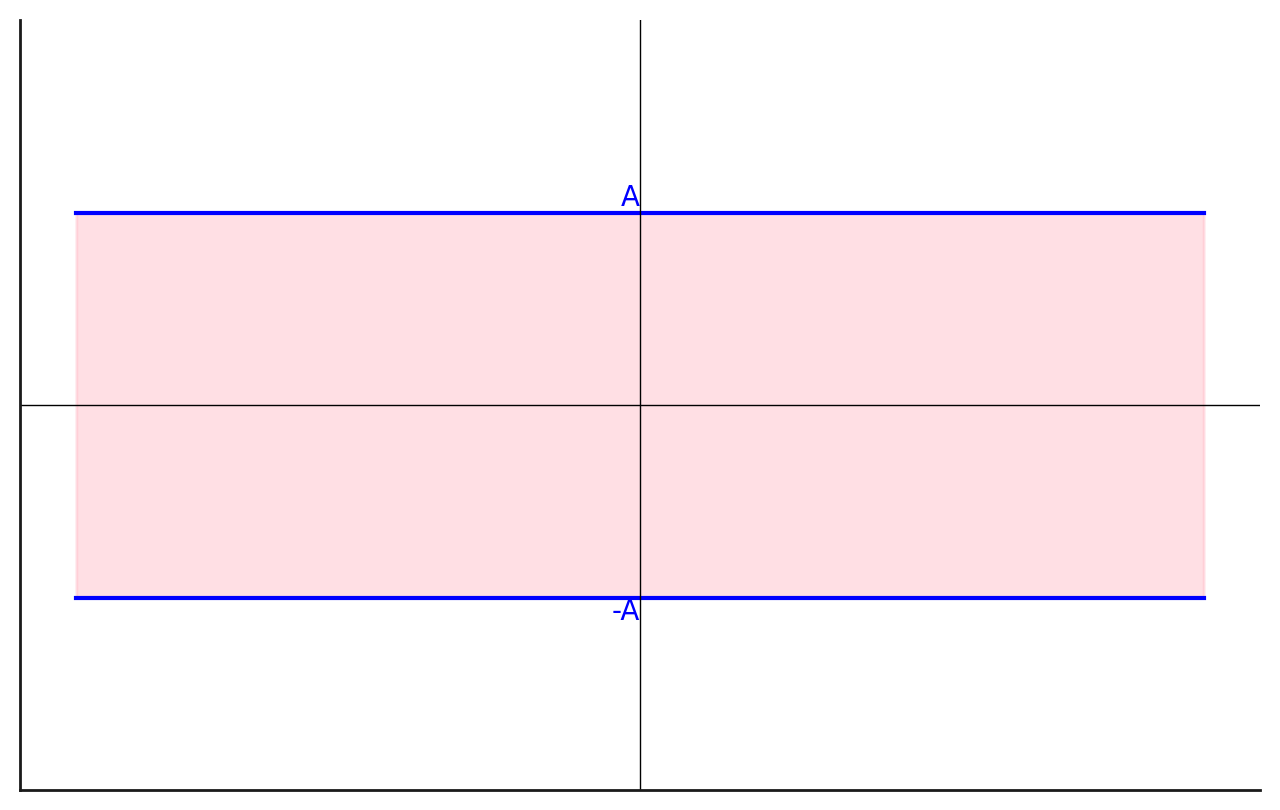
\includegraphics[width=0.5\linewidth]{Pictures/graph1.png}
%    \label{fig:graph1}
%\end{figure}

Таким образом, мы можем применить теорему Фубини к $F$ и получить для $\displaystyle \iint_{(-A, A) \times \R} F(y, u)dydu$ с одной стороны вот такое выражение:
\begin{multline*}
    \iint_{(-A, A) \times \R} F(y, u) du dy = \int_{\R} f(u) \int_{-A}^{A} e^{i(x - u)y}dy du = \\ =
    \int_{\R} f(u) \dfrac{e^{i(x - u)A} - e^{-i(x - u)A}}{i(x - i)}du = \int_{\R} f(u) \dfrac{2 \sin A(x - u)}{x - u}du = \int_{\R} f(x - t) \dfrac{2 \sin At}{t}dt.
\end{multline*}
А с другой стороны:
\begin{equation*}
    \iint_{(-A, A) \times \R} F(y, u) du dy = \int_{-A}^{A} e^{ixy} \int_{\R} f(u) e^{-iuy}du dy = \sqrt {2\pi} \int_{-A}^{A} \mathcal{F}[f](y) e^{ixy} dy = 2\pi I_A[f](x).
\end{equation*}
Если мы приравняем эти выражения и поделим на $2\pi$, то мы получим утверждение леммы:
\[
    I_{A}[f](x) = \int_{\R} f(x - t) \dfrac{\sin At}{\pi t}dt.
\]
\end{proof}

\begin{definition}
    Пусть $f \in L_1^{loc}(\mathbb{R})$.
\[
\text{Если } \exists \lim_{A \to +\infty} I_A[f](x) \text{ при } x \in \mathbb{R}, \text{ то говорят, что $\exists$ интеграл Фурье функции } f. 
\]

\begin{remark}
    По сути интеграл Фурье совпадает с $F^{-1}[F[f]].$
\end{remark}
\end{definition}

\begin{theorem}[Принцип локализации.]
    Пусть \( \widetilde{f} \in L_1([-\pi, \pi]) \) и \(2\pi\)-периодична.
    Пусть \( f \in L_1(\mathbb{R}) \) и совпадает с \( \widetilde{f} \) в некоторой окрестности точки \( \underline{x} \in \mathbb{R} \).
    Тогда следующие утверждения эквивалентны:
    \begin{enumerate}
        \item[$\bullet$] Интеграл Фурье функции $f$ в точке \(\underline{x}\) сходится;
        \item[$\bullet$] Ряд Фурье функции \(\widetilde{f}\) сходится в точке \(\underline{x}\).
    \end{enumerate}
    Более того, в случае наличия сходимости справедливо равенство:
\[
\frac{1}{\sqrt{2\pi}}\,\vpint
_{-\infty}^{+\infty}
\mathcal{F}[f](y)\,e^{\,i x\,y}\,dy
\;=\;
\sum_{n\in\mathbb{Z}}
c_{n}\bigl(\widetilde{f}\bigr)\,e^{\,i n x}.
\]
\end{theorem}

\begin{proof}

Докажем, что 
\[
I_A \bigl[f\bigr](\underline{x}) - S_{[A]}\bigl[\widetilde{f}\bigr](\underline{x}) \longrightarrow 0, \quad A \to +\infty, \text{ где $[A]$ - целая часть числа $A$}
\]

Из ключевой леммы (\ref{lem:key}) следует, что $I_A[f](\underline{x}) = \int\limits_{\mathbb{R}} f(\underline{x} - t) \frac{\sin(At)}{\pi t} \, dt$

Предположим, что $f \equiv \widetilde{f}  
    \text{ в } U_\delta(\underline{x})$ 
Заметим, что по теореме Римана об осцилляции $\forall S > 0 \hookrightarrow$
\[
I_A \left[ f \right](\underline{x}) = \int\limits_{-S}^{S} f(\underline{x} - t) \cdot \frac{\sin(At)}{\pi t} \, dt + o(1), \quad A \to +\infty
\]

С другой стороны, у нас есть следующая формула для частичных сумм ряда Фурье:

\[
S_n \left[\widetilde{f}\right](x) = \int\limits_{-\pi}^{\pi} \widetilde{f}(\underline{x} - t) \frac{\sin(nt)}{\pi t} \, dt + \varepsilon_n \left[\widetilde{f}\right](\underline{x})
\]

По теореме Римана об осцилляции: % ссылка со 2 лекции
\begin{gather*}
    S_n \left[\widetilde{f}\right](x) = \int\limits_{-\pi}^{\pi} \widetilde{f}(\underline{x} - t) \frac{\sin(nt)}{\pi t} \, dt + \varepsilon_n \left[\widetilde{f}\right](\underline{x}) = \int\limits_{-\delta}^{\delta} \widetilde{f}(\underline{x} - t) \frac{\sin(nt)}{\pi t} \, dt + o(1), \quad n \rightarrow +\infty\\
\end{gather*}
Если $A \in \Z$, то $I_A[f](\underline{x}) - S_{[A]}(\widetilde{f})(\underline{x}) = o(1)$ -- в силу совпадения функций в некоторой окрестности.
В общем случае, когда $A$ ~---~ нецелое, мы можем посмотреть на целую часть $A$
(вспомним, что $I_A$ ~---~ это интеграл от преобразования Фурье).
\[
\left| I_A \left[ f \right] (\underline{x}) - I_{[A]} \left[ f \right] (\underline{x}) \right| 
\leq 
\int\limits_{A-1}^{A} \left| \mathcal{F} [f](y) \right| \, dy + 
\int\limits_{A}^{A+1} \left| \mathcal{F} [f](y) \right| \, dy
\leq 2 \sup_{|y| \geq A-1} \left| \mathcal{F} [f](y) \right| \longrightarrow 0, \quad A \rightarrow +\infty
\]
Действительно, по теореме Римана об осцилляции (которую мы можем применить, поскольку по условию $f \in L_1(\R)$)
\[
\mathcal{F} \left[ f \right](y)  = \frac{1}{\sqrt{2 \pi}} \int\limits_{\mathbb{R}} f(y) \, e^{-ixy} \, dy \longrightarrow 0, y \longrightarrow \infty
\]
Используем неравенство треугольника и получим
\[
\begin{aligned}
\bigl|I_{A}[f](\underline{x}) - S_{[A]}[f](\underline{x})\bigr|
 \leq
\bigl|I_{A}[f](\underline{x}) - I_{[A]}[f](\underline{x})\bigr| + \bigl|I_{[A]}[f](\underline{x}) - S_{[A]}[f](\underline{x})\bigr|.
\end{aligned}
\]

Первое слагаемое $\bigl|I_{A}[f](\underline{x}) - I_{[A]}[f](\underline{x})\bigr| \rightarrow
 0, A \rightarrow +\infty$ из только что показанной оценки, а второе слагаемое стремится к нулю поскольку при $A \in \Z$ верно, что $I_A[f]$ и $S_A[f]$ совпадают с точностью до $o(1)$ в некоторой малой окрестности $\underline{x}$.
\end{proof}
